\setlength{\parindent}{10ex}

\documentclass{article} \usepackage{graphicx}

\title{Vulnerability Auditing Through Live Stack Tracing} \author{Spencer
Powell} \date{\today}

\begin{document}

\maketitle

\section {Overview}

%Make a workflow figure clarify relationship between debugger and monitor which
%preceeds which?

%TODO: first make the graph; then we will explain it.

The overall workflow of our vulnerability detection toolkit is shown in
%Figure\ref{fig-workflow}
Figure 1.1 and includes four main components: the stack monitor, which monitors
and logs stack activiy, the debugger, which calls functions within a target
program, a fuzzer, which supplies constructed random inputs to the program, and
a pattern detector, which uses machine learning to analyze the newly created
stack monitor logs and detect vulnerable code patterns. After the stack monitor
invokes the debugger, the debugger will call functions within the program
itself, in an effort to lessen the amount of code executed and increase the path
coverage. The debugger is capable of giving arguments to the given function,
which can be randomized by fuzzing. Fuzzing is a method of crafting random
inputs for a program in an effort to explore all paths within a given binary or
function. Previously known fuzzing techniques can be applied to these functions,
in an effort to trigger crashes. Exploring all paths through a givent binary is
an important step in this process because a given vulnerability in a binary may
not be located within a commonly executed logic path. The stack monitor
maintains a log of stack activity during each execution, which is written to a
file. Each time the fuzzer provides a different input to the program, a new log
file is produced and saved. This collection of files is then sent to the
vulnerability detector. The detector uses machine learning to recognize
vulnerable patterns in stack activity, and tags potentially vulnerable sections
of machine code.

\begin{figure} \begin{center}
%\vspace{-0.3in}
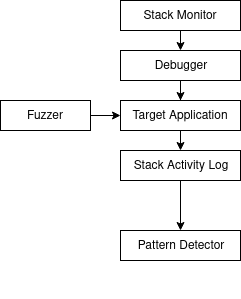
\includegraphics[height=4in]{workflow.png} \end{center}
%\vspace*{-0.3in}
\caption{The Overall Workflow}
%\vspace{-0.4in}
\label{fig-workflow} \end{figure}

\section{The Stack Monitor}

Our stack monitor serves to monitor the execution of an arbitrary program and
then creates a log of all the stack activities, which is later analyzed for
vulnerability detection. It takes as input a binary executable of a program
(currently only 64 bit x86 ELF's are supported). The monitor dynamically
instruments the user executable to log down the values of the runtime stack
pointer (SP), the base pointer for the stack (BP), and the instruction pointer
(IP) before each instruction is executed. If the instruction reads or writes to
memory, instrumentation is inserted to check whether the targeted memory is
within the runtime stack, and if yes, the memory operation is logged. All the
logged information is sent to the stack monitor from the instrumented binary
executable using a client-server model for interprocess-communication.
%An example of the logged information for ??? is illustrated in
%Figure~\ref{fig-logfile}.
The stack monitor can be configured to either output all the logs into an
external file, or in an internal data structure that can be accessed through
python.

% TODO: create figure for stack monitor

\section{The Binary Debugger}

The binary debugger provides an programming interface for the developer to
invoke the stack monitor to track any selected regions of code.  TODO: what is
the interface (API)? make a figure and reference the figure. Then try to explain
the logisitics of the API.

\begin{figure} \begin{center}
%\vspace{-0.3in}
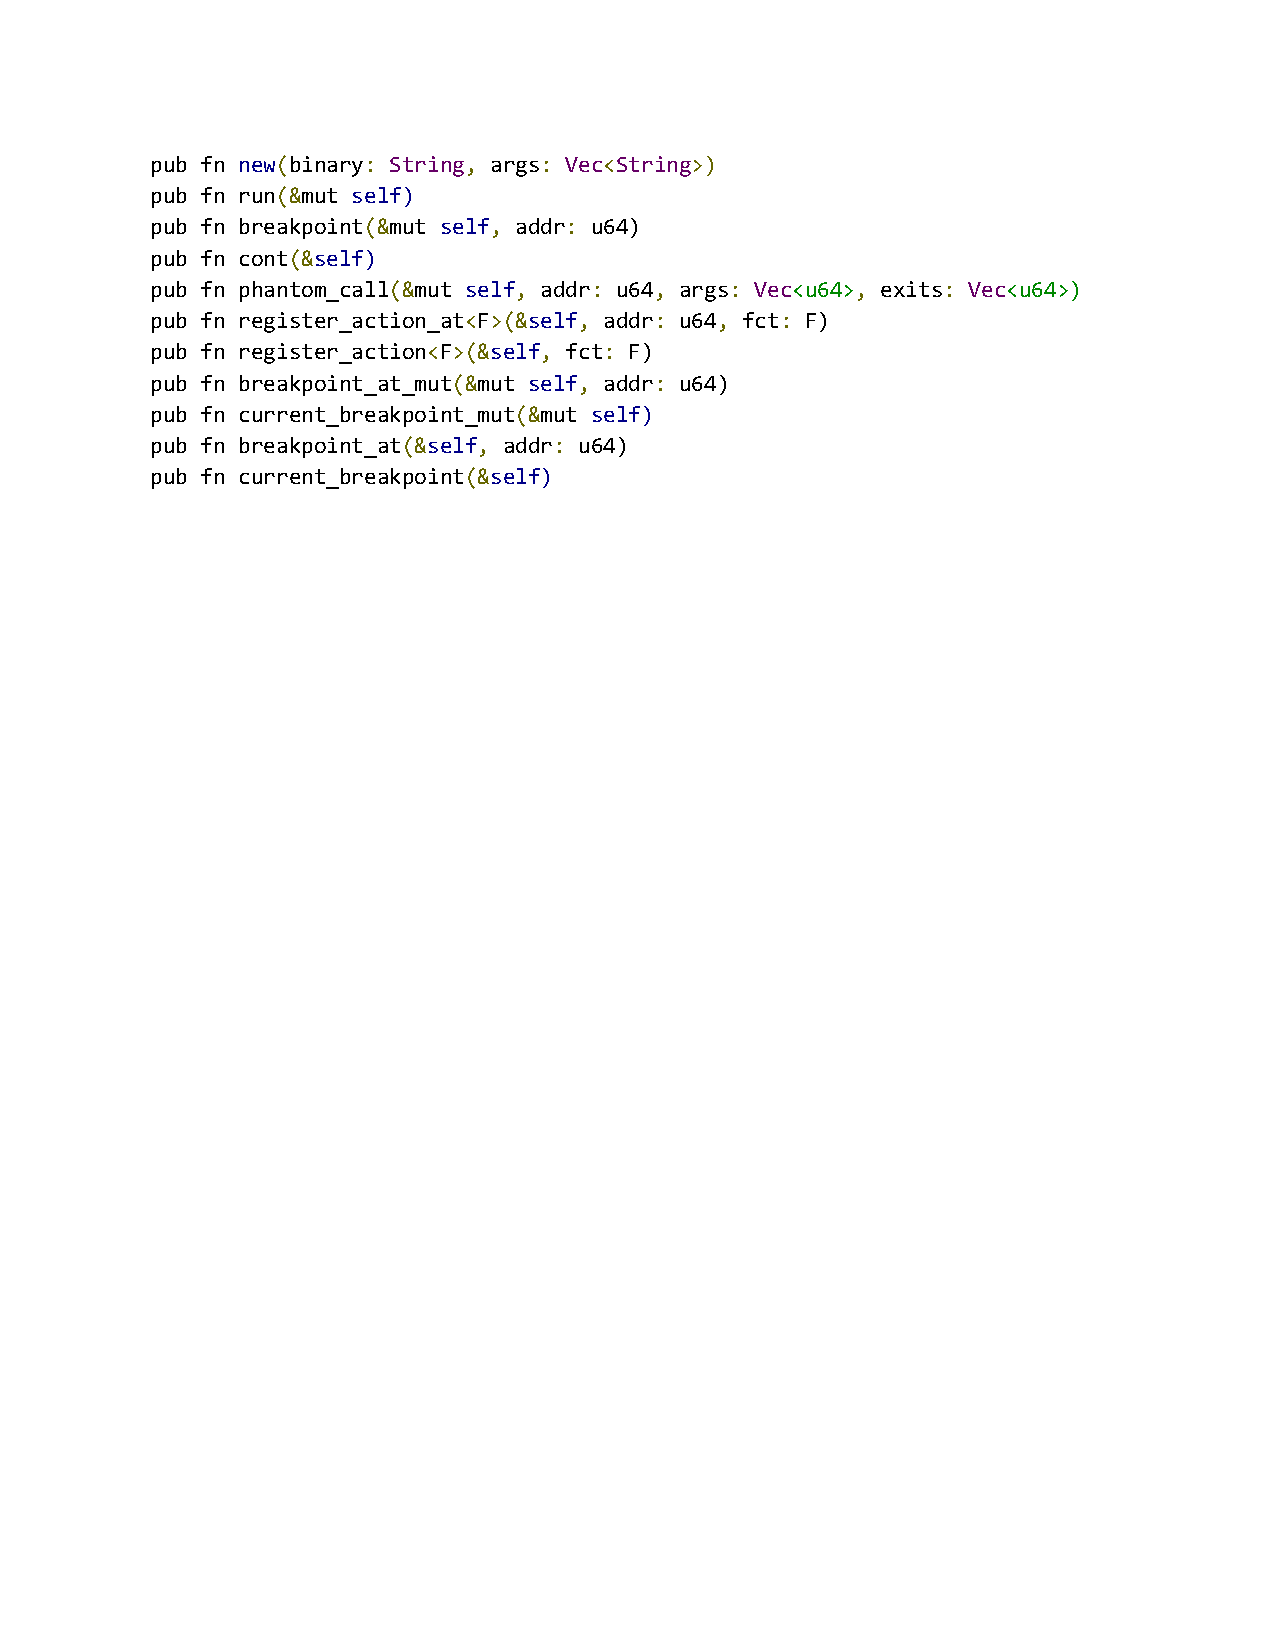
\includegraphics[height=4in]{api.pdf} \end{center}
%\vspace*{-0.3in}
\caption{The Debugger API}
%\vspace{-0.4in}
\label{fig-workflow} \end{figure}

The API works by allowing the user to set and manipulate breakpoints, and inject
false function calls dynamically anywhere in the code. The new() function
creates the debugger. The breakpoint() function sets a breakpoint in the code at
the given address. The user may optionally elect to add a callback function
which will be executed upon halting at a breakpoint with the register_action()
function. Similarly, the user may also create a callback for a specific
breakpoint using the register_action_at() function. The run() function spawns a
child process, which will be controlled by the debugger process. Upon arriving
at a breakpoint, the user may continue with the cont() function. At any
breakpoint, the user may also use the phantom_call() function. This function
takes an address, a list of arguments, and a list of exits. The address is
jumped to as if it were the start to a function. The arguments are placed into
the processes memory in accordance with the System V x86_64 calling convention,
which places arguments in RDI, RSI, RDX, RCX, R8, R9, and the pushes to the stack if
more arguments remain. The list of exits is a list of addresses which will be
considered as function returns. Breakpoints are placed at each exit
automatically, and each breakpoint is registered with a callback function which
will reset the programs registers to their original values.

TODO: provide an example of using the API of debugger in the fuzzer. Also the
figure will be used to explain the fuzzer.


The programming interface in Figure?? is implemented by making system calls to
ptrace. The ptrace systemcall works by taking four arguments. The first argument
is an enumerated request, which can represent a variety of actions. The second
argument is a process id (PID), which represents the "tracee" (the procress
whose memory is being manipulated). The third argument is an address, and is
only used for certain requests. The final argument is a void pointer to data,
which is also only used for certain requests. Both addr and data have different
meanings based on the chosen ptrace request. The debugger spawns a child tracee
process by first invoking the fork system call. The child process which results
from the fork call then performs an initial ptrace system call, using the
PTRACE_TRACEME request. This enables the child process to be traced by a parent
tracer process. Breakpoints are set using algorithm shown in % figure xxx

TODO: the specific ptrace call (with interface), TODO: explain how the ptrace
interface work. In particular, the debugger invokes ptrace with the TODO {what
requests} to allow the user to monitor and edit the memory of any child process,
to set breakpoints in a child, and to call any function in the child.

The function calls can be constructed with arguments, but no initialization is
done to global data. This can be a potential issue for processes which rely on
global variables or preallocated memory. Fake allocations can be performed by
manually allocating space on the stack before calling, but currently the only
fix for global variables is to partially execute sections of the program before
executing the desired code.


\section {Path Exploring} Dynamic execution has a few issues with it that must
be dealt with. One of the biggest issues with dynamic execution traces is that
of code coverage. Identifying a vulnerability requires that you first execute
the vulnerable piece of code. We have elected to use fuzzing as a technique for
code coverage, as it is well researched and there are many pre-existing methods
with which to explore a binary.

\section {The Vunerability Detection} The data from the monitor is analyzed
through machine learning, the data must be preprocessed. The addresses of the
stack operations are made to be relative to the base pointer, and the stack
frame is given in an overall size instead of both a stack and base pointer.

\section{Key Technical Challenge}

The key technical challenge of this tool is handling the massive amount of data.
Per instruction, the log contains three addresses, and extra optional data for
memory operations on the stack. This pressents two major issues. The first issue
is the massively increased runtime of the target binary which is required in
order to generate the information, and the second issue is comprehending and
manipulating the massive amount of data which is created.

The large influx of data is handled in two distinct methods. The first method is
a binary debugger which attempts to extract and call a given function from a
binary. This allows us to limit our scope of analysis to a single area, and
create multiple logs based on differing inputs. The second method used to handle
the large dataset is machine learning. Our goal is to discover patterns in stack
behavior could indicate vulnerable logic in a binary. There is far too much data
for this to be done manually, so machine learning was applied.

\end{document}
